\chapter{Differentially Private Decision Trees}

Differentially private decision tree learning methods aim at preventing information leakage at two levels: when splitting internal nodes, and when querying leaf nodes for prediction results. In \cite{fletcher_survey}, Fletcher et al. (2020) survey differential privacy methods for decision tree learning. They identify the main factors that need to be considered when designing such algorithms: 

\begin{itemize}
	\item \textbf{The privacy budget $\epsilon$}.
	\item \textbf{The number of times the data needs to be queried}. This directly impacts budget consumption. If the data needs to be queried multiple times, then we must apply the sequential composition theorem (Theorem ~\ref{theorem:sequential_composition}). It is clear from the theorem that the more queries there are, the faster the privacy budget will be consumed. The querying strategy of a differentially private model is therefore crucial.
	\item \textbf{The sensitivity $\Delta$ of the queries}. For a fixed privacy objective, tighter sensitivity bounds lead to less added noise, as shown in Theorem ~\ref{theorem:lap} and ~\ref{theorem:exp}: in the Laplace mechanism, reducing the sensitivity $\Delta f$ will reduce the scale of the associated Laplace distribution, hence decreasing the amount of added noise. Equally, in the exponential mechanism, reducing the sensitivity $\Delta u$ will make sure that the chosen attribute's value has a high probability of being amongst the best possible choices.
	\item \textbf{The size of the dataset}. The larger the dataset is, the easier it is for the trees to learn the underlying data structure (since they have access to more data to make better splits), and the least sensitive to noise the trees will be (since a large amount of data will make sure that best splits are chosen with high probability).
\end{itemize}

\section{Related work}

In this section, we explore current and past related work.

\subsection{Privacy budget allocation}\label{sec:budget_allocation}

Jagannathan et al. (2009) \cite{jagannathan} are amongst the first ones to propose a practical differentially private implementation of decision trees for classification problems. They propose a differentially private version of the ID3 algorithm, and show that a naive implementation where counting queries are noised lead to very poor utility under realistic privacy budget constraints. In fact, splitting a privacy budget of $\epsilon=1$ evenly across all queries achieves a classification error rate as high as $81.27\%$ on the nursery dataset\footnote{\href{https://archive.ics.uci.edu/ml/datasets/nursery}{https://archive.ics.uci.edu/ml/datasets/nursery}}. To address this shortcoming, they propose a new approach based on \textit{Random Forest} ensemble methods. Instead of adding noise to each of the queries made during the ID3 algorithm, the decision trees are computed at random and noise is only added to the leaf nodes. This leads to tremendous improvements, with the previously reported error rate dropping to approximately $10.5\%$ for the same dataset and under similar privacy constraints. For comparison, the non-private version of the ID3 algorithm achieves an error rate of $1.81\%$ on the same dataset.

In \cite{mohammed}, Mohammed et al. (2011) split the privacy budget $\epsilon$ into two halves, where each is used for the internal nodes and the leaf nodes respectively ($\epsilon_{node} = \epsilon_{leaf} = \frac{\epsilon}{2}$). Rather than selecting the splitting attribute using noisy counts as in \cite{jagannathan}, Mohammed et al. (2011) propose to use the exponential mechanism (as defined by Theorem ~\ref{theorem:exp}). The main advantage of using the exponential mechanism to select the splitting attribute is that it exponentially favours candidates with a high information gain, hence building more accurate decision trees. In \cite{liu}, Liu et al. (2018) propose to split $\epsilon$ into $s_i$ shares for the selection of internal nodes, based on the $k^{th}$ harmonic number: $s_i = \frac{1}{k} + \frac{1}{k-1} + \dots + 1$. Denoting the budget share for leaf nodes by $s_l = 1$, the total number of shares is $s_t = s_i + s_l$. With $k$ being a fixed, pre-defined number of attributes, Liu et al. (2018) assign $\epsilon_{node} = \frac{\epsilon}{s_t} * \frac{1}{k^2}$ and $\epsilon_{leaf} = \frac{\epsilon}{s_t}.$ Under these constraints, the decision tree satisfies $\epsilon$-differential privacy. We refer the reader to \cite{liu} for a formal analysis of the budget allocation. With the above budget allocation strategies and under Theorem ~\ref{theorem:sequential_composition}, building an ensemble of $T$ decision trees requires a total privacy budget of $\epsilon T$. This means that if the privacy target is $\epsilon$, and because of the data overlap amongst the trees, each tree only receives  a privacy budget of $\epsilon_{t} = \frac{\epsilon}{T}$. As $T$ grows bigger, trees therefore only receive a very small privacy budget, leading to high noise addition and poor accuracy.

Fletcher et al. (2017) \cite{fletcher_smooth} and Li et al. (2020) \cite{dpgbdt} address this shortcoming by proposing an ensemble of trees where each tree operates on a distinct subset of the data. Under these new constraints, each tree within the ensemble can use the full privacy budget: $\epsilon_{t} = \epsilon$. However, this approach doesn't work well on small datasets. Indeed, since every tree operates on its own subset of data, the total number of instances that each tree receives becomes smaller as the number of trees grows bigger. Consider a dataset of $n$ instances $\textbf{X} = X_1,\dots,X_n$ and an ensemble of $T$ trees. Each tree gets roughly $n_{tree} = \ceil{\frac{n}{T}}$ instances. If $T$ is too small, then the learning algorithm suffers from the pitfalls outlined in Section ~\ref{section:decision_trees}. If $T$ is too high, then $n_{tree}$ is small and the decision trees might not have enough instances to learn the underlying structure of the dataset.

In \cite{wen_wang} and \cite{nazanin}, the authors mention an adaptive budget allocation method. Rather than fixing an equal privacy budget used at each depth of the tree, the authors propose to compute this quantity during the tree induction algorithm. In the former case, the budget at each depth $d$ is computed as $\epsilon_{node} = \frac{1}{2^d}\epsilon_{t}$. This exponentially decaying budgeting is motivated by the intuition that early splits in the tree are more important than subsequent splits, hence why they get a higher portion of the privacy budget. However, such an allocation method might not be ideal when the tree gets very deep, as lower levels in the tree will receive a really small budget, which in turn creates too much noise and penalizes the quality of the tree. In the latter, the author proposes a new induction algorithm, \textit{ADiffP-$\phi$}, that computes each split's privacy budget dynamically and uses it as a termination criteria when the budget gets too small. Thus, the total number of nodes in the tree is not controlled by the maximum depth (or any other usual termination criteria), but by the total privacy budget available to the tree.

\subsection{Query sensitivity}\label{sec:query_sensitivity}

Fletcher and Islam (2015) \cite{fletcher_local} explore reducing the sensitivity of the splitting functions, hopping to reduce the amount of noise added in the tree-building process. Rather than computing the global sensitivity of a function, they propose to compute the local sensitivity of the Gini index in the node being split as $\Delta = 1 - (\frac{n_i}{n_i + 1})^2 - (\frac{1}{n_i + 1})^2$ where $n_i$ is the support of node $i$ (the support is equal to the number of instances in the node). This sensitivity reduction directly improves the Laplace and exponential mechanisms, as a tighter sensitivity bound allows for lower added noise. However, in its current form, this sensitivity derivation might be too noisy in some cases and incorrectly providing differential privacy. The same authors later proposed additional work (\cite{fletcher_signal}, \cite{fletcher_smooth}) based on Nissim et al. (2007) \cite{nissim}'s smooth sensitivity definition to enhance their model.

In \cite{dpgbdt}, Quinbin et al. (2020) propose a new way to bound the sensitivity of both the leaf nodes and the splitting function. Using new procedures (\textit{Geometric Leaf Clipping} and \textit{Gradient-based Data Filtering)}, they proved that the sensitivity of the leaf nodes could be bound by $\Delta V \leq \min(\frac{g_l^*}{1 + \lambda},2g_l^*(1-\eta)^{t-1})$ and that the sensitivity of the splitting function could be bound by $\Delta G \leq 3g_l^{*2}$, where $g_l^*$ is the maximum possible 1-norm gradient, $\lambda$ is a regularisation parameter, $\eta$ is the learning rate and $t$ is the index of the tree being constructed. These new bounds offer better accuracy in the differentially private settings.

Wang et al. (2020) \cite{wen_wang} introduce the first provably accurate privacy preserving, top-down decision tree learning algorithm in the distributed setting. More information about top-down algorithms can be found in \cite{kearns}. They propose a new splitting function, \texttt{PrivateSplit}, that approximates the optimal split chosen by the top-down algorithm, while providing differential privacy and proving boosting-based utility guarantees. In fact, they show that their algorithm only needs $(1/\epsilon)^{O(\log(1/\epsilon)/\gamma^2)}$ splits to achieve a training error $\leq \epsilon$ with probability $\geq 1-\delta$ (provided that the dataset has a certain size). On the adult dataset\footnote{\href{https://archive.ics.uci.edu/ml/datasets/adult}{https://archive.ics.uci.edu/ml/datasets/adult}}, their algorithm achieves roughly $79\%$ accuracy, which is a little over Quibin et al. (2020) \cite{dpgbdt}'s accuracy (roughly $74\%$) over the same dataset and under the same privacy budget constraints $\epsilon = 1$.

\subsection{Termination criteria and post-processing}

When building a decision tree, one must choose some criteria as to when to stop growing the tree. The simplest criterion is to stop growing the tree once it reaches a certain depth $d$. Other termination criteria include defining a maximum number of leaf nodes that a tree can have, or defining a minimum number of samples that a node must have before being split (i.e. a minimum node support). However, there is no optimal value for any of these criteria that works for every dataset. Rather, it is left to the user to find appropriate values that work best for their use case. In some cases, these parameters may be estimated based on the dataset. In \cite{fan}, the authors limit the tree depth to $d = \frac{k}{2}$ where $k$ is the number of features in the dataset. In \cite{jagannathan}, the tree depth is set to $d = \min(k/2, \log_b(n) - 1)$ where $n$ is the size of the dataset, and $b$ is the branching factor.

Once the tree has reached its termination criteria, one can apply post-processing methods, such as \textit{pruning}, to the tree. Pruning consists in removing untrustworthy leaf nodes from the tree. A leaf node can be considered untrustworthy if its support or purity (homogeneity of the class labels in the node) is too low. In the differentially private settings, pruning cannot be applied as it is in traditional decision trees, as the modifications to the tree induction algorithm induced by differential privacy need to be accounted for. Friedman and Schuster (2010) \cite{friedman_schuster} adapt classical pruning mechanisms by normalising the support of each node in the tree, so that that sum of all counts in all nodes matches the size of the dataset (which is not initially the case due to the noise introduced by differential privacy). In random forests, Fletcher and Islam (2015) \cite{fletcher_signal} observe that in some cases, an additional split worsens the decision tree rather than help it, since the split is chosen at random. They therefore propose to prune leaf nodes where the added noise is greater than the class count signal.

\subsection{Depth-first and best-leaf first decision tree induction}\label{sec:growth}

There are several ways to grow a decision tree during its induction process. While most algorithms grow trees by level, i.e. depth-wise, some implementations (like XGBoost \cite{xgboost}) grow decision trees with a best-leaf first approach. This approach was first described by Haijian S. (2007) \cite{shi} in his doctoral thesis. Figure ~\ref{fig:tree_dfs} and ~\ref{fig:tree_bfs} show the differences between a depth-first and a best-leaf first tree induction algorithm (the figures are adapted from XGboost documentation\footnote{\href{https://github.com/Microsoft/LightGBM/blob/master/docs/Features.rst}{https://github.com/Microsoft/LightGBM/blob/master/docs/Features.rst}}).

\begin{figure}[h!]
	\center
	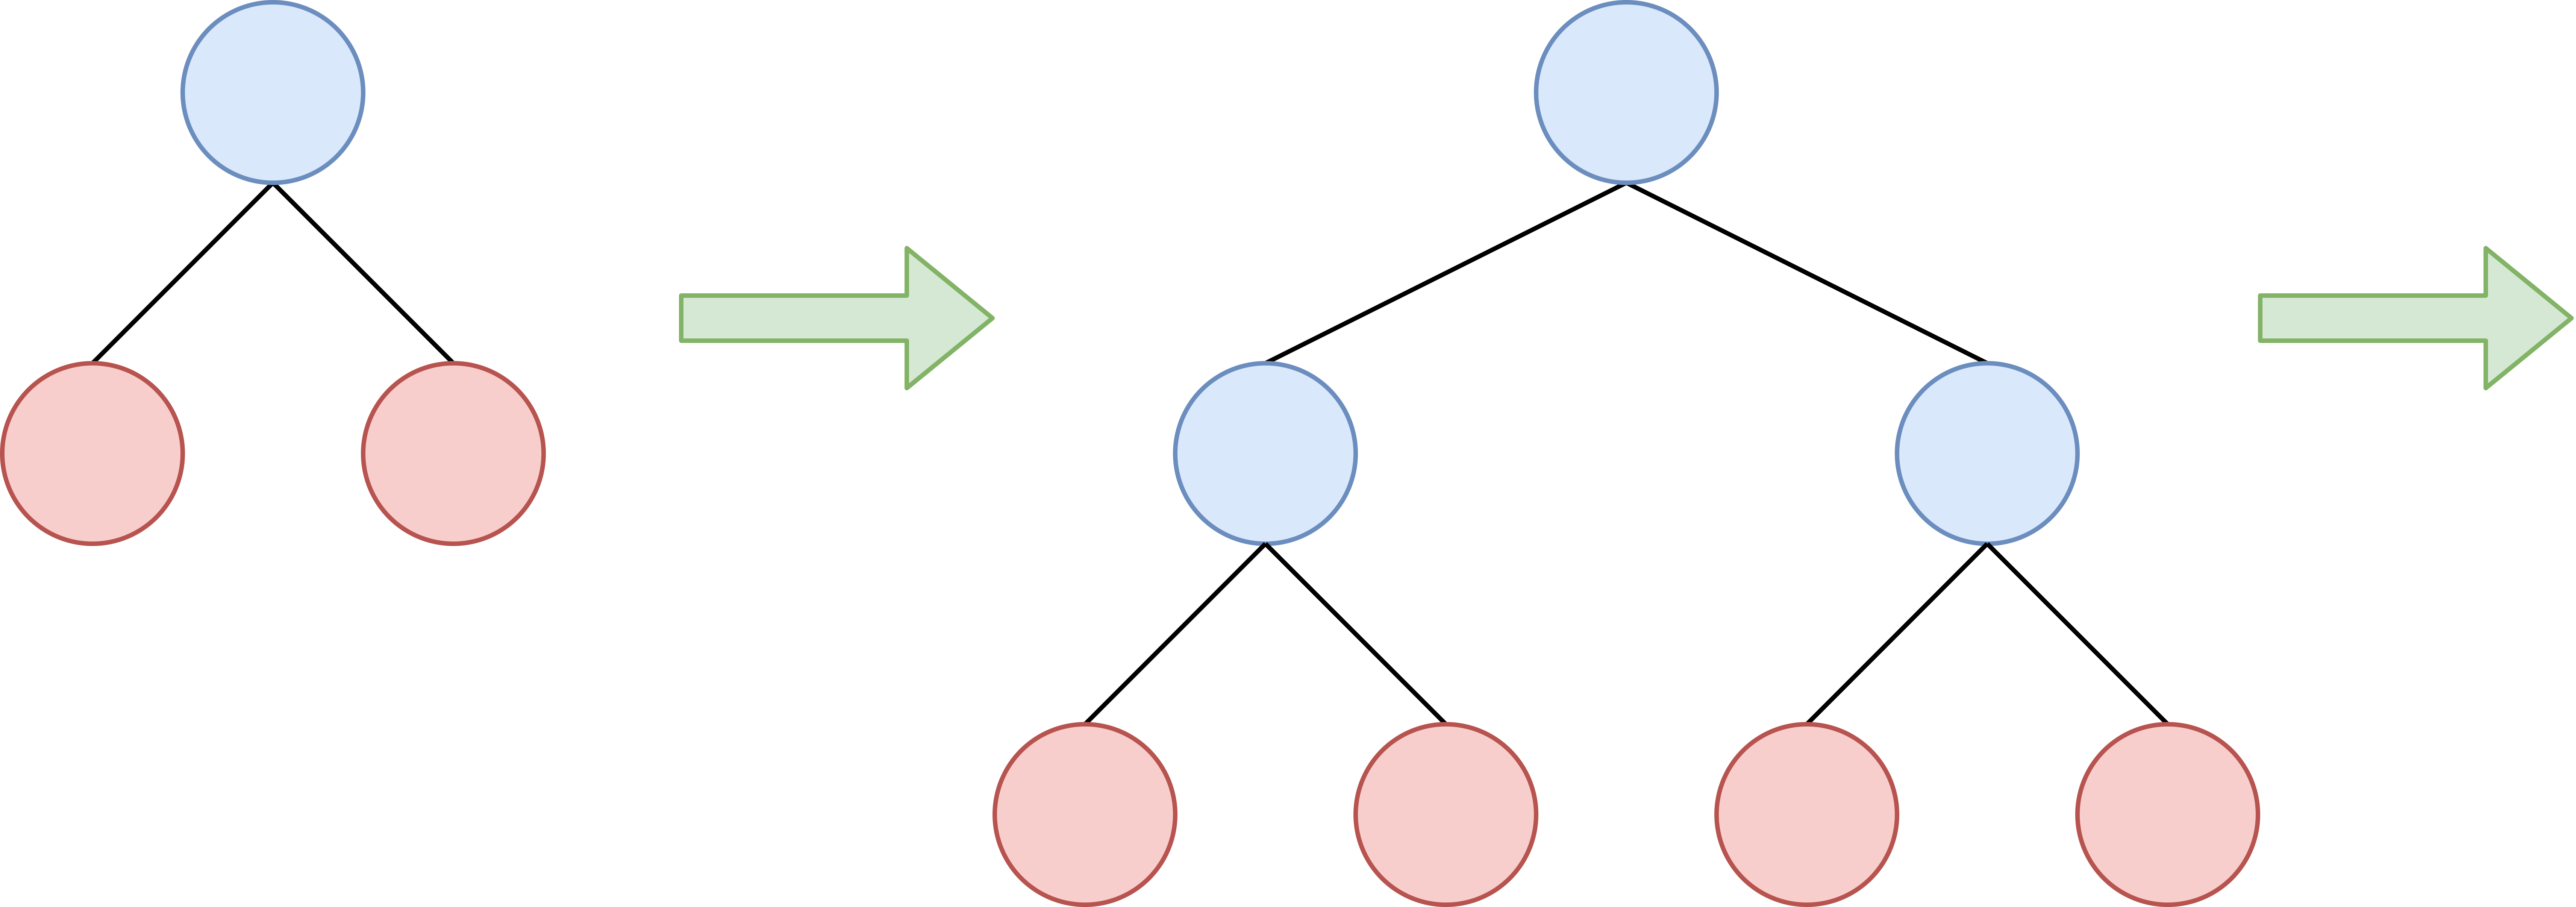
\includegraphics[scale=0.7]{images/dpgbdt/dfs}
	\caption{\label{fig:tree_dfs} A depth-first decision tree induction algorithm.}
\end{figure}

\begin{figure}[h!]
	\center
	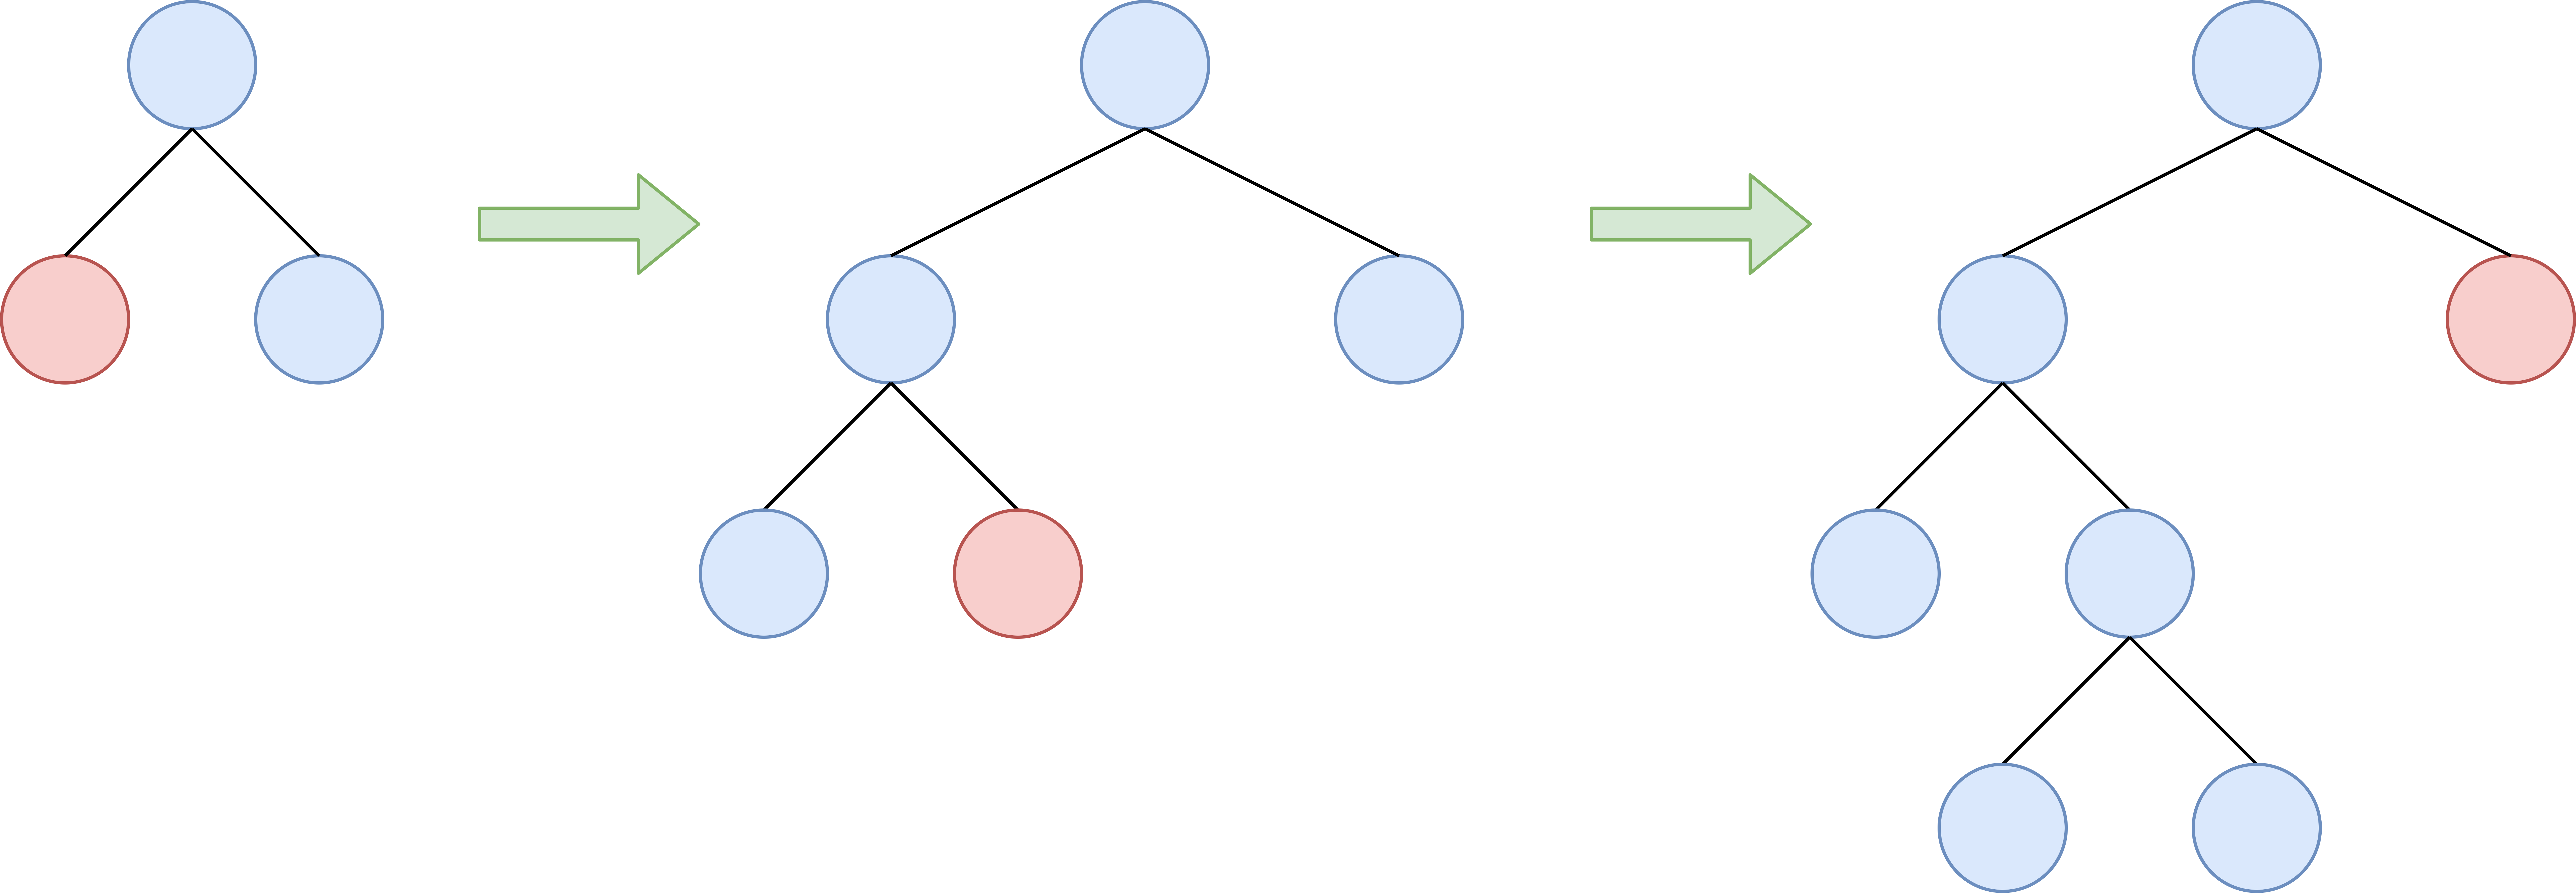
\includegraphics[scale=0.7]{images/dpgbdt/bfs}
	\caption{\label{fig:tree_bfs} A best-leaf first decision tree induction algorithm.}
\end{figure}

Depending on the dataset, a best-leaf first induction might achieve a lower loss. However, when the number of data is small, a best-leaf first approach may over-fit the dataset. 

In the next section, we choose to explore in more details the work of Quibin et al. (2020) \cite{dpgbdt}. This choice is motivated by the tight sensitivity bounds that the authors were able to derive, along with the good prediction accuracy that their model showed.


\section{Differentially private gradient boosted decision trees (DP-GBDT)}

To make decision trees differentially private with the definitions provided in Section ~\ref{sec:dp}, the literature (\cite{inprivate}, \cite{mohammed}, \cite{dpgbdt}) proposes two changes to Algorithm ~\ref{algo:gbdt}:
\begin{itemize}
	\item For each node, the attribute and the attribute's value on which the node is split must be chosen through the exponential mechanism. The information gain $G$ is used as the utility function, and the exponential mechanism guarantees that the attributes and attributes' value with higher gain have a higher probability of being chosen.
	\item For each leaf node, the leaf value must be noised through the Laplace mechanism.
\end{itemize}

Qinbin et al. (2020) \cite{dpgbdt} suggests that each tree $t$'s privacy budget $\epsilon_t$ gets split into two parts: $\epsilon_{leaf} = \frac{\epsilon_t}{2}$ for the leaf nodes and $\epsilon_{node} = \frac{\epsilon_t}{2d_{max}}$ for the internal nodes, where $d_{max}$ is the maximum depth for the tree $t$. Since the nodes in one depth have disjoint inputs, Theorem ~\ref{theorem:parallel_composition} can be applied and the privacy budget in one depth needs to be counted only once. Thus, the total privacy budget consumption is no more than $\epsilon_{node} * d_{max} + \epsilon_{leaf} = \epsilon_t$. Once a tree is trained, the gradients of all instances are updated. This allows the next tree to converge towards a minimum for the objective function defined in Equation ~\ref{eq:gbdt_obj}. The authors propose Algorithm ~\ref{algo:dp_gbdt}.

\begin{algorithm}
	\DontPrintSemicolon
	\SetKwComment{Comment}{$\triangleright$\ }{}
	\SetCommentSty{itshape}
	\caption{Differentially private GBDTs training process \cite{dpgbdt}}\label{algo:dp_gbdt}
	\KwIn{$\textbf{X} = X_1,\dots,X_n$: instances, $\textbf{y} = y_1, \dots, y_n$: labels}
	\KwIn{$\lambda$: regularisation parameter, $d_{max}$: maximum depth, $\eta$: learning rate}
	\KwIn{$T$: total number of trees, $l$: loss function, $\epsilon$: privacy budget}
	\KwOut{An ensemble of trained differentially private decision trees.}
	$\epsilon_t$ = $\epsilon$ \ \Comment*[r]{\textcolor{blue}{Each tree is trained on a disjoint subset of the dataset, so we can apply Theorem ~\ref{theorem:parallel_composition}}}
	\For{$t=1$ \textbf{to} $T$}{
		Update gradients of all training instances on loss $l$ \;
		$\epsilon_{leaf} = \frac{\epsilon_t}{2}, \; \epsilon_{node} = \frac{\epsilon_t}{2d_{max}} $ \;
		\For{d = 1 \textbf{to} $d_{max}$}{
			\For{\textit{each node in current depth}}{
				\For{\textit{each split value i}}{
					$G_i \gets \frac{(\sum_{i \in I_L}g_i)^2}{|I_L| + \lambda} + \frac{(\sum_{i \in I_R}g_i)^2}{|I_R| + \lambda}$ \Comment*[r]{\textcolor{blue}{Equation ~\ref{eq:gbdt_gain_simplified}}}
					$P_i \gets \exp(\frac{\epsilon_{node} \cdot G_i}{2 \Delta G})$ \Comment*[r]{\textcolor{blue}{Theorem ~\ref{theorem:exp}}}
				}
				Split node on split value $i$, where $i$ is chosen with probability $P_i / \sum_j P_j $
			}
		}
		\For{\textit{each leaf node i}}{
			$V_i \gets \eta \left(-\frac{\sum_{i \in I}g_i}{|I| + \lambda} + Lap(0, \Delta V/\epsilon_{leaf}) \right)$ \Comment*[r]{\textcolor{blue}{Equation ~\ref{eq:gbdt_leaf_value} and Theorem ~\ref{theorem:lap}}}
		}
	}
\end{algorithm}

The authors use the parallel composition theorem (Theorem ~\ref{theorem:parallel_composition}) to lower the privacy budget consumption by training each decision tree on a disjoint set of data. However, when the training dataset is small and the number of trees is large, each tree only gets very few samples to learn from. This low number of samples available to the trees results in bad splits, which damages the quality of the trees and their predictions. To address this limitation, we propose in the next chapter a new induction algorithm, \textit{2-nodes}.
